% Diagram: Decoder-only Architecture with Layer Detail
\begin{figure}[htbp]
\centering
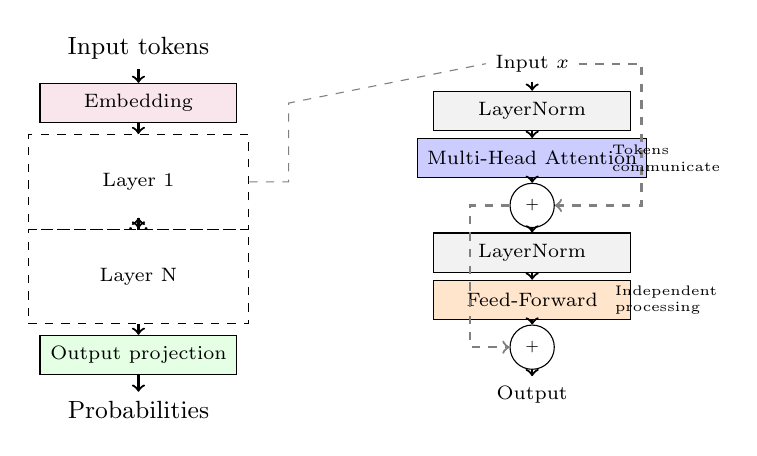
\begin{tikzpicture}[
    node distance=0.5cm,
    block/.style={rectangle, draw, minimum width=2.5cm, minimum height=0.5cm, font=\scriptsize},
    attn/.style={block, fill=blue!20},
    ffn/.style={block, fill=orange!20},
    norm/.style={block, fill=gray!10},
    arrow/.style={->, thick}
]
% Left side: Overall architecture
\node (input) {\small Input tokens};
\node[block, fill=purple!10, below of=input, yshift=-0.2cm] (emb) {Embedding};

% Simplified layers
\node[rectangle, draw, dashed, minimum width=2.8cm, minimum height=1.2cm, below of=emb, yshift=-0.5cm] (l1box) {};
\node at (l1box.center) {\scriptsize Layer 1};

\node[below of=l1box, yshift=-0.1cm] (dots) {...};

\node[rectangle, draw, dashed, minimum width=2.8cm, minimum height=1.2cm, below of=dots, yshift=-0.1cm] (lnbox) {};
\node at (lnbox.center) {\scriptsize Layer N};

\node[block, fill=green!10, below of=lnbox, yshift=-0.5cm] (out) {Output projection};
\node[below of=out, yshift=-0.2cm] (probs) {\small Probabilities};

% Left arrows
\draw[arrow] (input) -- (emb);
\draw[arrow] (emb) -- (l1box);
\draw[arrow] (l1box) -- (dots);
\draw[arrow] (dots) -- (lnbox);
\draw[arrow] (lnbox) -- (out);
\draw[arrow] (out) -- (probs);

% Right side: Layer detail (expanded view)
\node[right of=l1box, xshift=4.5cm, yshift=1.5cm] (layer-input) {\scriptsize Input $x$};

% Attention block
\node[norm, below of=layer-input, yshift=-0.1cm] (ln1) {LayerNorm};
\node[attn, below of=ln1, yshift=-0.1cm] (attn) {Multi-Head Attention};

% First residual
\node[circle, draw, fill=white, minimum size=0.3cm, below of=attn, yshift=-0.1cm] (add1) {\tiny +};

% FFN block
\node[norm, below of=add1, yshift=-0.1cm] (ln2) {LayerNorm};
\node[ffn, below of=ln2, yshift=-0.1cm] (ffn) {Feed-Forward};

% Second residual
\node[circle, draw, fill=white, minimum size=0.3cm, below of=ffn, yshift=-0.1cm] (add2) {\tiny +};

\node[below of=add2, yshift=-0.1cm] (layer-output) {\scriptsize Output};

% Detail arrows
\draw[arrow] (layer-input) -- (ln1);
\draw[arrow] (ln1) -- (attn);
\draw[arrow] (attn) -- (add1);
\draw[arrow] (add1) -- (ln2);
\draw[arrow] (ln2) -- (ffn);
\draw[arrow] (ffn) -- (add2);
\draw[arrow] (add2) -- (layer-output);

% Residual connections
\draw[arrow, gray, dashed] (layer-input.east) -- ++(0.8,0) |- (add1.east);
\draw[arrow, gray, dashed] (add1.west) -- ++(-0.5,0) |- (add2.west);

% Annotations
\node[right of=attn, xshift=1.2cm, font=\tiny, align=left] {Tokens\\communicate};
\node[right of=ffn, xshift=1.2cm, font=\tiny, align=left] {Independent\\processing};

% Connection between left and right
\draw[dashed, gray] (l1box.east) -- ++(0.5, 0) -- ++(0, 1) -- (layer-input.west);

\end{tikzpicture}
\caption{Decoder-only transformer: N layers of attention + FFN with residual connections.}
\label{fig:decoder-only}
\end{figure}
